% INTRODUCTION CONTENT

\section{The cell}
The cell is the smallest unit of life, of which all known living organisms are composed. Every cell houses a plethora of biomolecular processes that allows it to continuously adapt to changes in its environment. Due to the dynamic nature of these processes, it can be very challenging to comprehend the cellular response to a signal. A reductionist approach to understanding a complex biological system is to study the biochemical components of which it is comprised\cite{brigandt_reductionismbiology_2017}.

Recent advances in experimental technologies are playing a crucial role in reductionist biology, allowing to measure the abundance of thousands of different biochemical molecules in tens of thousands of individual cells. With it comes the challenge of analysing large amounts of data that are not easily interpretable by hand. The sheer volume of the data generated from such highly-integrative and high-throughput experiments are not the only reason why they are so challenging to interpret. For instance, the generated data contains high levels of noise arising from inherent biomolecular stochasticity in the cells and from the experimental profiling techniques used, as well as batch effects arising from differences between donors and labs\cite{hon_humancellatlas_2018}. Biologists thus turn to computer scientists
to develop new tools to tackle these problems and help them to extract meaningful biological insights from the data. In this work, incremental contributions were made to the field in order to be able to address the aforementioned problems in a more comprehensive context.

Observing the biomolecular insides of cells can ultimately provide fundamental understanding into the processes that govern these cells and help uncover novel approaches for disease diagnosis, prognosis, and treatment. For example, the Human Cell Atlas (HCA) consortium\cite{regev_humancellatlas_2018} has set out to develop a comprehensive reference map of all the different types of cells in the human body. Experts in the field often metaphorically describe the HCA initiative as aiming to develop a 'Google Maps' of the human body. Even in its infancy, the HCA has profiled 3.8 million cells from 248 donors across 42 labs\cite{humancellatlasconsortium_humancellatlas_2018}, and this number is likely to increase well above one hundred million.

The next part of the chapter highlights several key concepts in both cell biology and computer science, upon which the remainder of this work relies.

\subsection{The origin of life and the RNA world}
The discovery of the double helix shape of deoxyribonucleic acid (DNA)\cite{watson_molecularstructurenucleic_1953} is often considered the pivot point in our understanding of the origin of life and evolution. By now, it is well known that DNA serves as a medium for storing the genetic information required to reproduce a whole organism. With other words, the DNA of an organism contains the complete set of instructions required to build all of the biomolecular machinery present in its body. 

Life (or cells) did not originate from DNA, however. A widely-accepted hypothesis states that life originates from its lesser-known cousin, ribonucleic acid (RNA). According to the RNA world hypothesis\cite{alberts_rnaworldorigins_2002}, the very first primitive cells used RNA both to store genetic information and to perform the chemical reactions required to sustain themselves (Figure \ref{fig:rnaworld}). Only later did cells develop the ability to use the more chemically stable DNA molecules to self-sustain in a process commonly referred to as the central dogma.

\begin{figure}[htb!]
	\centering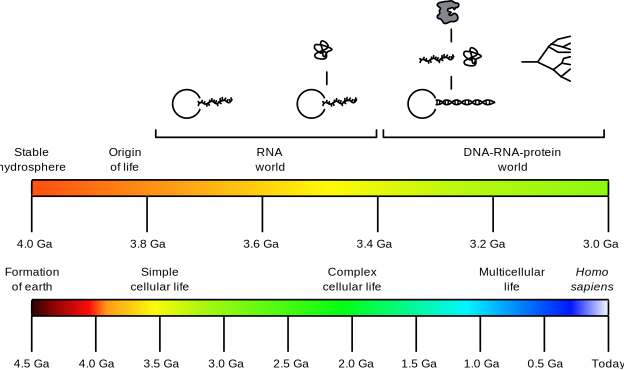
\includegraphics[width=.5\linewidth]{fig/rnaworld} % TODO: change image
	\caption{
		\textbf{RNA world.} The postulated rise and fall of the RNA world during the evolution of life, from early self-replicating RNA to complex, RNA-controlled metabolism, to the invention of translation, followed by diversification of all modern branches of life. Image from Horning (2011)\cite{horning_rnaworld_2011}.
		\fbox{\color{red} TODO: combine images, rewrite the description.}
	}
	\label{fig:rnaworld}
\end{figure}

\subsection{Central dogma}
The central dogma describes the general flow of genetic information in almost all existing living cells: DNA is decoded to RNA, which in turn encodes proteins\cite{strachan_humanmoleculargenetics_2011}. Main processes involved in the central dogma are \textbf{transcription}, \textbf{splicing}, and \textbf{translation} (Figure \ref{fig:centraldogma}). 

\begin{figure}[htb!]
	\centering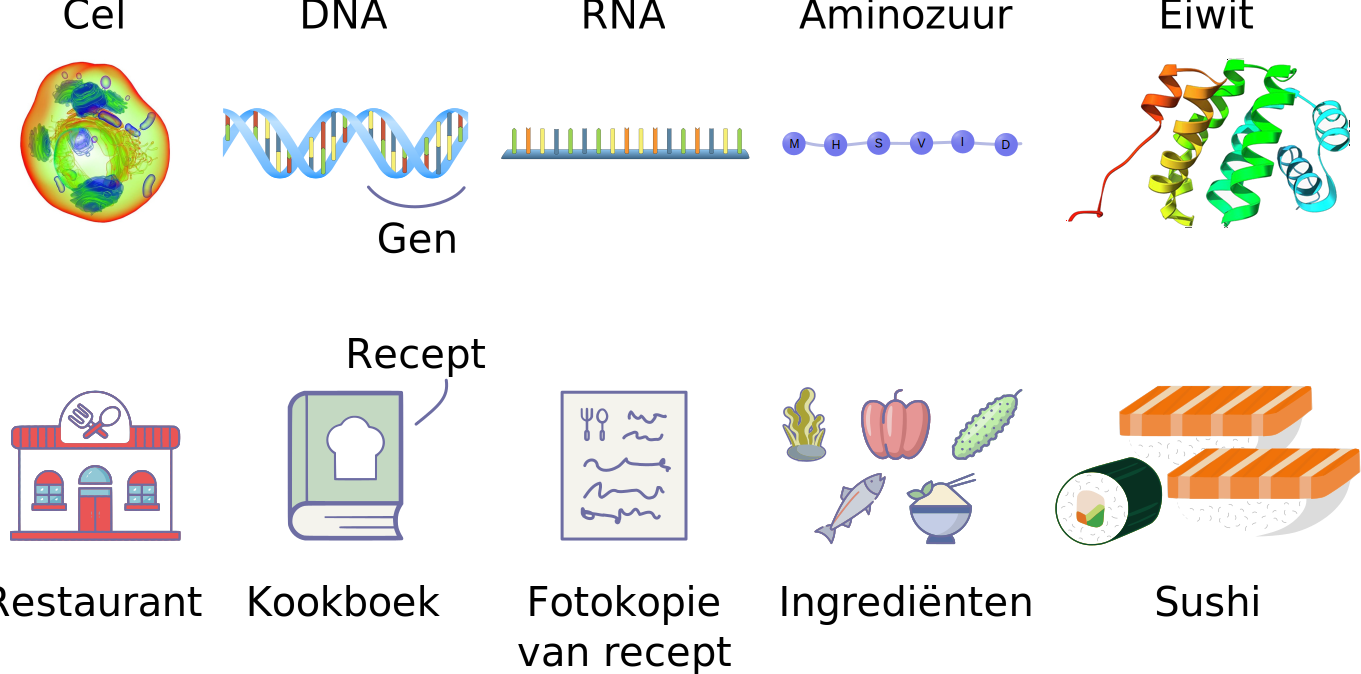
\includegraphics[width=.5\linewidth]{fig/central_dogma} % TODO: change image
	\caption{
		\textbf{Central Dogma.}
		\fbox{\color{red} TODO: combine images, rewrite the description.}
	}
	\label{fig:centraldogma}
\end{figure}

% KDP: je zegt niets over epigenetica, die min of meer bepaald welke gebieden in het DNA worden vertaald (dit leidt je misschien te ver...)
During the process of \textbf{transcription} that takes place in the cell nucleus, a complementary RNA copy is transcribed from the template DNA. The initial RNA transcript is a precursor messenger RNA (pre-mRNA) that needs to undergo series of maturation steps to ultimately form the mature messenger RNA (mRNA). This maturation includes pre-mRNA \textbf{splicing} to remove non-protein coding intervening sequences (the introns) and to join the neighbouring protein-coding sequences (the exons). A single pre-mRNA can be alternatively spliced to generate multiple forms of mRNAs that will result in the production of multiple protein isoforms. This process of alternative splicing is essential to generate more than 100'000 different proteins starting from just 20'000 genes\cite{nilsen_expansioneukaryoticproteome_2010}.

The mature mRNA is then transported to the cytoplasm, where it engages with ribosomes to initiate \textbf{translation}. During this highly evolutionary conserved process, a chain of amino acids, known as the protein building blocks, is being synthesised. Each amino acid is specified by three nucleotides (a codon) in the mRNA, according to a nearly universal genetic code. After being released by the ribosomes, the translation product undergoes a variety of chemical modifications to form the final folded protein, the structure of which is determined by the sequence of different amino acids in the chain. In addition, polypeptides may be cleaved to yield more than one active polypeptide product. The structure of a protein determines its functionality, which includes catalysing biochemical reactions, providing structure, and transportation of molecules.


\subsection{Cell types}
\textit{Homo sapiens} like to categorise everything they encounter, and so too have they conceptualised groups of cells called "cell types". The human body contains more than 200 different cell types that are classified into four groups: epithelial, connective, muscle, and nervous. This however, is a major underestimation of the real number of cell types. Neurons, for instance, that are known to be extremely diverse, are estimated to reach numbers above 10,000 different types\cite{strachan_humanmoleculargenetics_2011}.

The concept of cell types eases reasoning and our understanding about many aspects of biology (e.g. the process of cell differentiation, cell-cell communication, cellular response to certain stimuli). Some cells are known to be highly specialised toward performing a particular function (e.g. memory B cells accelerate immune response by remembering previously encountered pathogens), or they can maintain a strong ability to differentiate into other cell types.

One common approach for understanding the functionality of a particular cell is to observe which molecules are present in the cell and to associate those set of molecules with functionality. Taking a snap shot of the protein or RNA transcript content in a particular cell, might already provide us with major insights into its functionality. However, in order to fulfil a particular task, the biochemical machinery of the cell gradually changes over time. Therefore it is highly informative to also consider the transition states between cell types and the dynamic processes involved therein.

\subsection{Cell dynamics and gene regulation}
Cells are dynamic entities that can gradually produce the molecules needed to acquire new functionality. The naturally occurring cell-to-cell variability happens at the level of gene expression. Gene expression itself can be controlled at different levels (Figure~\ref{fig:controlexpression}), one of which is gene regulation by transcription.

\begin{figure}[htb!]
	\centering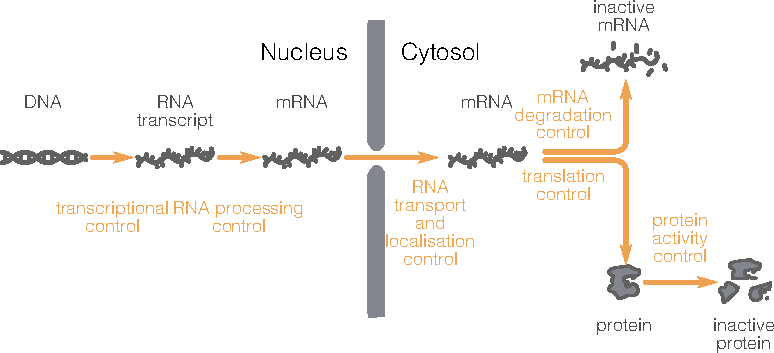
\includegraphics[width=.8\linewidth]{fig/control_gene_expression} % TODO: change image
	\caption{
		\textbf{Levels of controlling gene expression} can happen at the level of transcription, RNA processing (i.e. splicing), RNA transport and localization, mRNA translation, mRNA degradation and protein activity \cite{alberts_overviewgenecontrol_2002}.
	}
	\label{fig:controlexpression}
\end{figure}

According to the needs of a cell, different genes are being transcribed. Housekeeping genes are being expressed in essentially every cell, while other genes are cell type or tissue specific or may be expressed in response to developmental and environmental signals\cite{strachan_humanmoleculargenetics_2011}. 

Transcription factors (TFs) modulate the rate of gene transcription by binding and recruiting the transcriptional machinery to \emph{cis}-regulatory regions (enhancers, and silencers) that are typically located in the promotor region of target genes. These bindings may result in increased or decreased gene expression. 
There are several TF families of which members share structural characteristics (e.g. zinc finger, helix-loop-helix).

Many TFs are commonly present in virtually all cell types (e.g. NF-$\kappa$B), while others are specific for cells and developmental stages\cite{lambert_humantranscriptionfactors_2018}. Typically, the same TF can regulate the rate of transcription of many target genes in different cell types, indicating that these gene regulatory networks (GRNs) are dynamic. Moreover, the production of a specific molecule might require several gene regulatory cascades. Studying the active parts of a cell's GRN can thus reveal which dynamic processes are taking place within a cell.

% KDP: misschien interessant om over tumor heterogeniteit te spreken: waarvan we vroeger dachten dat homogene massa van cellen was, blijkt toch veel complexer te zijn --> nu mogelijk om met sc technieken te bestuderen?

\subsection{Profiling single cells}
Several technologies are now available to profile (i.e. observe) biomolecular components, allowing us to gain better understanding in the biological processes that take place within a cell. The single-cell "omics" technologies originated from the convergence of two different fields, \emph{"single-cell"} and \emph{"omics"}.

\subsubsection{Single-cell}
The earliest approach for measuring the abundance of a particular molecule in \emph{single cells} is the microscope.
Since its development by Coons et al. (1941), immunohistochemistry (IHC) has been instrumental in visualising proteins.\cite{coons_immunologicalpropertiesantibody_1941}. 
A cell can present a particular type of protein, also called an antigen, on its cell surface. In many multicellular organisms, antigens can stimulate the immune system to produce antibodies. IHC realises the visualisation of proteins by exploiting the principle of antibodies binding to specific antigens.

IHC (and many other biotechnologies) visualises antigen-antibody reactions by attaching particular molecules to the antibody, such as an enzyme that catalyses a colour-producing reaction, or a fluorescent chemical compound that can re-emit light upon excitation. The use of several colours (wavelengths) allows measuring expression levels of different antibodies simultaneously. Characterising cells in a semi-quantifiable way is labour intensive, however; since it involves acquiring an image of many cells and drawing a contour around each cell (called cell segmentation).
Modern implementations of IHC improve the throughput drastically by using robots and computer software to provide semi-automated image acquisition and cell segmentation\cite{theodosiou_automatedanalysisfish_2007}.

Flow cytometry\cite{fulwyler_electronicseparationbiological_1965} circumvents imaging and segmentation issues by running a steady stream of cells through a laser and measuring the amount of fluorescent light scattered from those cells. 
Since cells need to be suspended in a buffer, flow cytometry is particularly useful for analysing non-adherent cells such as the many different immune cells in blood. However, many protocols already exist to extract viable single cells from tissues and tumours\cite{leelatian_preparingviablesingle_2017}.
Conventional flow cytometry devices enable to measure protein expression levels of millions of cells using up to eight different antibody fluorochromes simultaneously, while state-of-the-art instrumentation allows detection of up to 27 biomarkers simultaneously\cite{cossarizza_guidelinesuseflow_2017}.

Besides IHC and flow cytometry, many new technologies have been developed which allow quantifying expression levels of molecules in single cells (e.g. mass cytometry, single-cell quantitative polymerase chain reaction, fluorescence \emph{in situ} hybridization). All of these single-cell (non-omics) technologies are limited by the number of different molecules they measure, however. Selecting molecules of interest prior to analysis, makes the experiment biased towards the preconceptions of the experimenter.

\subsubsection{Omics}
On the other side of the spectrum are the so-called "omics" technologies. "Omics"\footnote{The etymology of "omics" is quite interesting\cite{yadav_wholenesssuffixomics_2007}.} is a collective term for profiling all molecules of a particular type in a high-throughput manner.
There are many types of "omics", such as genomics, transcriptomics and proteomics. Genomics studies the complete DNA sequence of an organism's genome, while transcriptomics and proteomics study the RNA transcripts and proteins, respectively.

Specific examples of omics technologies are whole genome sequencing to determine the DNA sequence of an organism, and RNA sequencing to profiles the sequence of RNA transcripts, both using next-generation sequencing technologies. A gene expression profile can be obtained by mapping the sequences of RNA transcripts to the genome.

Several high-throughput technologies have been developed to investigate proteomes in depth. The most commonly applied are mass spectrometry-based and gel-based techniques (e.g. differential in-gel electrophoresis).

% Je had proteomics technieken niet meer aangehaald. -> zie deze paperlink voor eventueel fig 1 of 2. Hoewel dit misschien niet je hoofdtopic is. https://academic.oup.com/chromsci/article/55/2/182/2333796

Typically for these methods, to capture enough material to generate a profile, numerous cells need to be pooled and lysed together, thereby granting the technology's name "bulk" omics.
Bulk omics is a major workhorse in molecular genetics and has applications in cancer research and in diagnostic screening of inheritable disorders.

Increasing evidence shows that cells are biomoleculary heterogeneous, even in very similar cell types\cite{hwang_singlecellrnasequencing_2018} (Figure~\ref{fig:bulk_vs_sc}A). Since a bulk profile is a population average (or rather, a summation), important cell-to-cell variability is not discernible (Figure~\ref{fig:bulk_vs_sc}B). 

\begin{figure}[htb!]
	\centering
	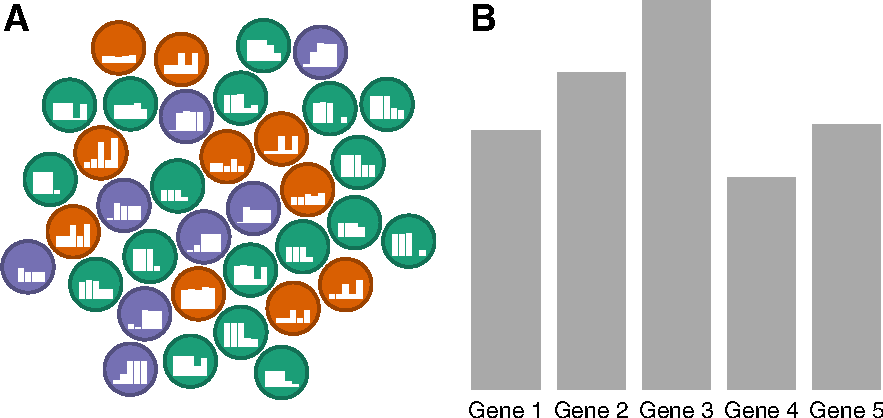
\includegraphics[width=\LARgefigure]{fig/bulk_vs_sc} 
	\caption{
		\textbf{The 'masking' effect of bulk omics.} 
		\textbf{A:} Cells from several subpopulations are incorrectly assumed to be homogeneous and are profiled with a single bulk omics experiment.
		\textbf{B:} The signals from the different subpopulations are masked. The resulting profile is dissimilar from the majority of cells it is supposed to represent.
	}
	\label{fig:bulk_vs_sc}
\end{figure}

\subsubsection{Single-cell omics}
Comparing single-cell technologies with omics technologies shows that they have both clear advantages but also significant drawbacks (Figure \ref{fig:profiling_convergence}A). Single-cell biology allows profiling thousands or even millions of cells, but only for a select number of genes. On the other hand, omics biology provides a broader view -- since genes do not need to be selected beforehand -- but is a profile of ensemble of cells and thus masks important cellular heterogeneity.

Advances in microvolume sequencing allowed profiling the transcriptome at single-cell resolution, thereby bringing single-cell biology and omics together to create single-cell omics. During the decade that followed, the number of single-cell omics technologies has sky-rocketed, allowing to profile >100'000 cells\cite{svensson_exponentialscalingsinglecell_2018} and measuring other levels of information (e.g. protein abundance and spatial location) \cite{moudgil_multimodalscrnaseq_2019}.

\begin{figure}[htb!]
	\centering
	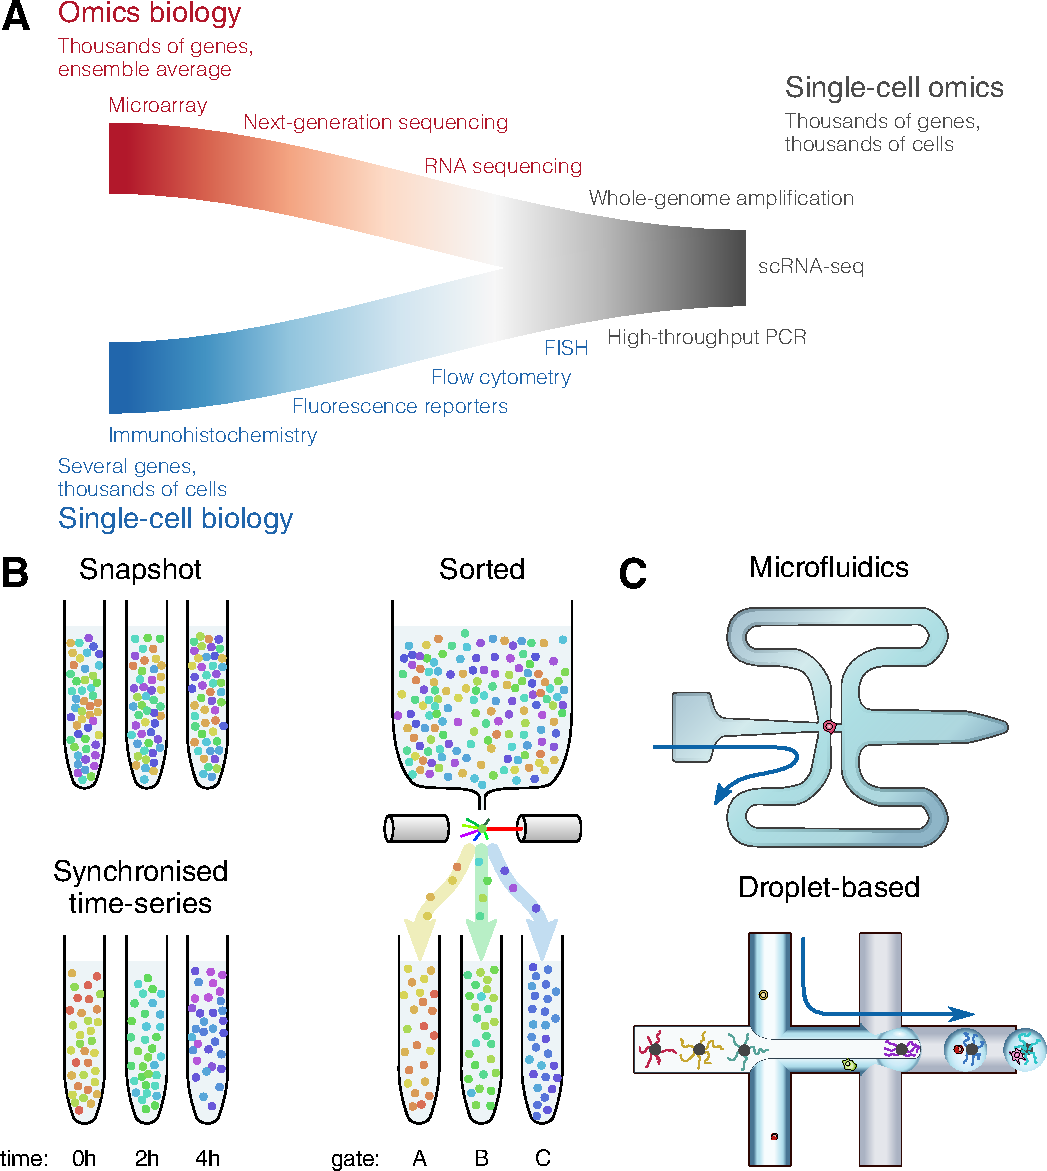
\includegraphics[width=.7\linewidth]{fig/scomics_2.pdf} 
	\caption{
		\textbf{A:} Convergence of single-cell and omics biology.
		\textbf{B:} Different approaches for sampling cells with decreasing levels of cellular heterogeneity within the different sub-populations: snapshot, time-series, sorted.
		\textbf{C:} Two common single-cell RNA sequencing technologies. Microfluidics systems let cells travel through nanometer scale tubing, capturing individual cells at intersections. Droplet-based systems encapsulate individual cells in droplets.
	}
	\label{fig:profiling_convergence}
\end{figure}

% could be expanded with information on how to isolate single cells and how to profile them
% see https://www.nature.com/articles/s12276-018-0071-8
% seems interesting as well: 10.1146/annurev-biodatasci-080917-013452

In this work, unless noted otherwise, we will be working with transcriptomics data resulting from a single-cell RNA-sequencing experiment (scRNA-seq). The workflow of generating scRNA-seq profiles is as follows. Same as other single-cell (non-omics) profiling methods, cells first need to be isolated (Figure~\ref{fig:profiling_convergence}B). Different sampling techniques yield different levels of information about cellular state. By now, many protocols for extracting and tagging RNA from single cells have been developed\cite{svensson_exponentialscalingsinglecell_2018}, the most popular of which are based on microfluidics or droplets (Figure~\ref{fig:profiling_convergence}C). By sequencing the trancripts and the attached unique cell identifier tags, each read can be mapped and tallied up. scRNA-seq data can thus be summarised in a matrix, where each column represent a single cell, each row a gene, and each value represents the number of transcripts that were sequenced for that gene and cell.

The rapidly advancing field of single-cell omics harbours exceptional opportunities to discover new aspects of biology and redefine existing knowledge. Some of these opportunities lie in efforts like the HCA consortium. They have set out to redefine all human cell types in both terms of their gene expression and location, and as well as the developmental trajectories connecting the different cell types. As part of this endeavour, the consortium will likely profile the whole transcriptomes of tens or even hundreds of millions of cells. 

\section{Computational tools}
Whole-genome profiling at single-cell level allows new types of analyses with which to study cellular heterogeneity at a hitherto unseen throughput. 
The new types of analyses permitted by single-cell omics present several computational challenges\cite{stegle_computationalanalyticalchallenges_2015, yuan_challengesemergingdirections_2017, chen_singlecellrnaseqtechnologies_2019}. This necessitates the development of novel computational tools, either because the problem statement of the performed analysis is completely novel, or to adapt existing methodology to new data characteristics -- dimensionality and noise. 

scRNA-seq data is typically very sparse -- while the human genome has more than 20'000 genes, they only contain non-zero values of a few thousand genes (typically <4'000). This is partially due to cells being specialised in particular functions and thus they do not need proteins of every time, but also due to RNA transcription occurring in bursts rather than continuously\cite{nicolas_whatshapeseukaryotic_2017}. This contributes to the high levels of noise seen in scRNA-seq data: no two cells have the same set of non-zero genes. 

Over the past five years, already 450 new tools have been developed to perform various analyses of single-cell omics data\cite{zappia_exploringsinglecellrnaseq_2018}, taking into account the specific noise characteristics. The most frequent types of analyses are detailed in the following subsections.

\subsection{Dimensionality reduction}
Single-cell omics datasets are usually one or more high-dimensional matrices, containing between M = $10^3$ to $10^5$ cells and typically about N = $10^3$ to $10^4$ genes (Figure~\ref{fig:comp_tools_dimred}A). The dimensionality of such datasets is typically too high for humans to interpret manually and for most modelling algorithms to tackle directly. 
Moreover, in reality, the intrinsic dimensionality of biological systems is probably much lower. For example, a differentiating hematopoietic cell could be described by just three dimensions: the first two dimensions lays out the hematopoietic lineage tree, and a third dimension allows for reprogramming between branches to occur.

Dimensionality reduction (DR) methods transform high-dimensional data into a meaningful low-dimensional representation. DR methods have two main target audiences; computers -- to construct a K-dimensional (with K $\ll$ M) representation of the data such that pairwise distances between different samples are retained as well as possible (Figure~\ref{fig:comp_tools_dimred}B); and humans -- to obtain a visual overview of the data (Figure~\ref{fig:comp_tools_dimred}C).

Each dimension frequently corresponds to one or more modules of co-expressed genes.  The reduced space can be interpreted in way analogous to Waddington’s epigenetic landscapes\cite{waddington_strategygenesdiscussion_1957,ferrell_bistabilitybifurcationswaddington_2012,rebhahn_animatedlandscaperepresentation_2014}, where the landscape dictates the possible states a cell can reside in, and transitions between states correspond to dynamic cellular processes, such as cell differentiation. 

\begin{figure}[htb!]
	\centering
	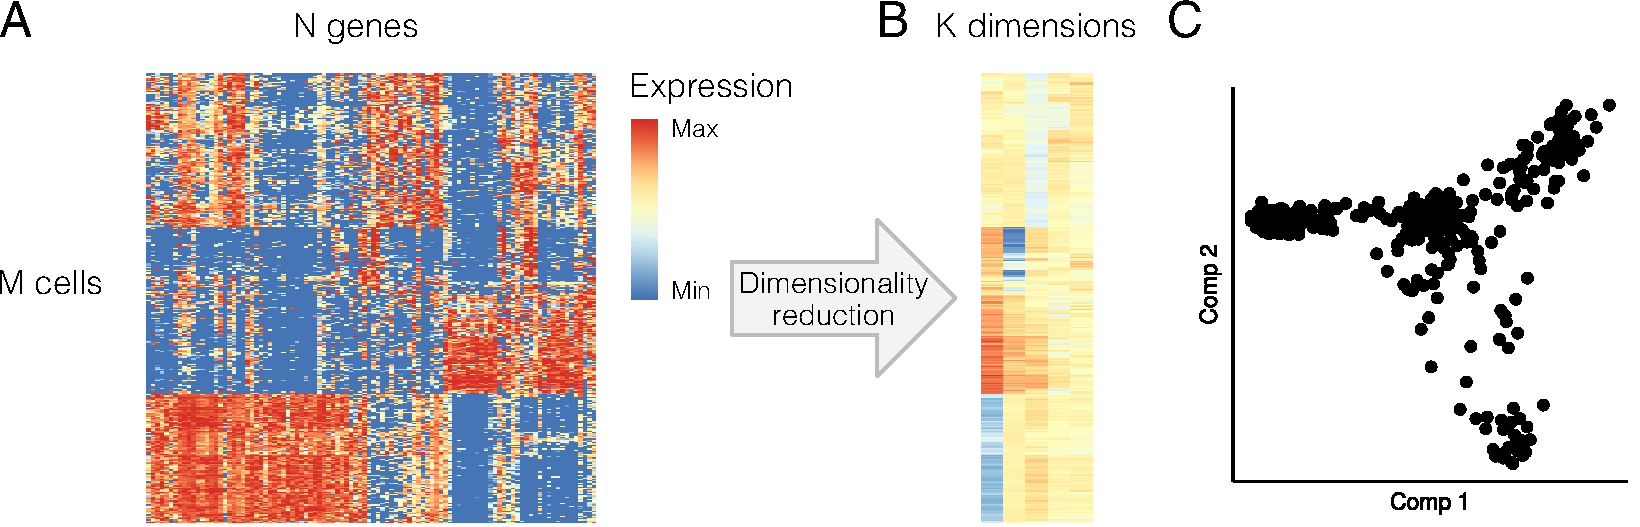
\includegraphics[width=\linewidth]{fig/comptools2/comptool_1_dimred.pdf} 
	\caption{
		\textbf{Dimensionality reduction for single-cell omics data.}
		\textbf{A:} A heatmap visualisation of an scRNA-seq expression dataset of fibroblasts being reprogrammed to neuron cells\cite{treutlein_dissectingdirectreprogramming_2016}. Only the most variable 
		\textbf{B:} The reduced space is a M$\times$K-dimensional matrix which attempts to conserve the cellular heterogeneity of the original space as well as possible.
		\textbf{C:} A dot plot of the first two components of the reduced space provides a global overview of the cells in the dataset. Colouring the dots according to prior information (e.g. cell type) or gene expression provides insight into the cellular heterogeneity within the dataset.
	}
	\label{fig:comp_tools_dimred}
\end{figure}

DR methods can be classified into two main categories, feature projection-based and manifold learning\cite{engel_surveydimensionreduction_2012}. 

Projection-based DR methods aim to perform a transformation of the data while preserving the pairwise distances between samples as much as possible. Examples of commonly used projection-based DR methods in single-cell omics are Principal Component Analysis\cite{pearson_liiilinesplanes_1901} (PCA) and Multi-Dimensional Scaling\cite{kruskal_multidimensionalscalingoptimizing_1964} (MDS). 

Manifold learning DR methods reconstruct a higher-order structure in the original space (e.g. a graph or a grid), visualising the structure in a lower-dimensional space, and mapping the original samples to the lower-dimensional space. Manifold learning can be an iterative optimisation process using a predefined criterion. Examples of manifold learning techniques are t-distributed Stochastic Neighbor Embedding\cite{vandermaaten_visualizingdatausing_2008} (t-SNE), Diffusion Maps\cite{nadler_diffusion_2005,coifman_diffusionmaps_2006} and Uniform Manifold Approximation and Projection\cite{mcinnes_umapuniformmanifold_2018} (UMAP). 

For scalability reasons, this work mostly makes use of Landmark MDS\cite{silva_globallocalmethods_2002,lee_landmarkmdsensemble_2009} (LMDS) with a Spearman rank correlation distance metric. LMDS is an extension of classical MDS, but rather than calculating a complete distance matrix between all pairs of cells, a set of landmark cells is sampled, only the distances between a set of landmarks and the samples are calculated. 

\subsection{Clustering}
To learn about the different cellular states within a population of cells, clustering methods divide up the cells into separate groups of highly similar cells (Figure~\ref{fig:comp_tools_cluster}A). 
By visualising gene expression of known genes involved in the cell types of interest, the clusters can be annotated (Figure~\ref{fig:comp_tools_cluster}B). 

\begin{figure}[htb!]
	\centering
	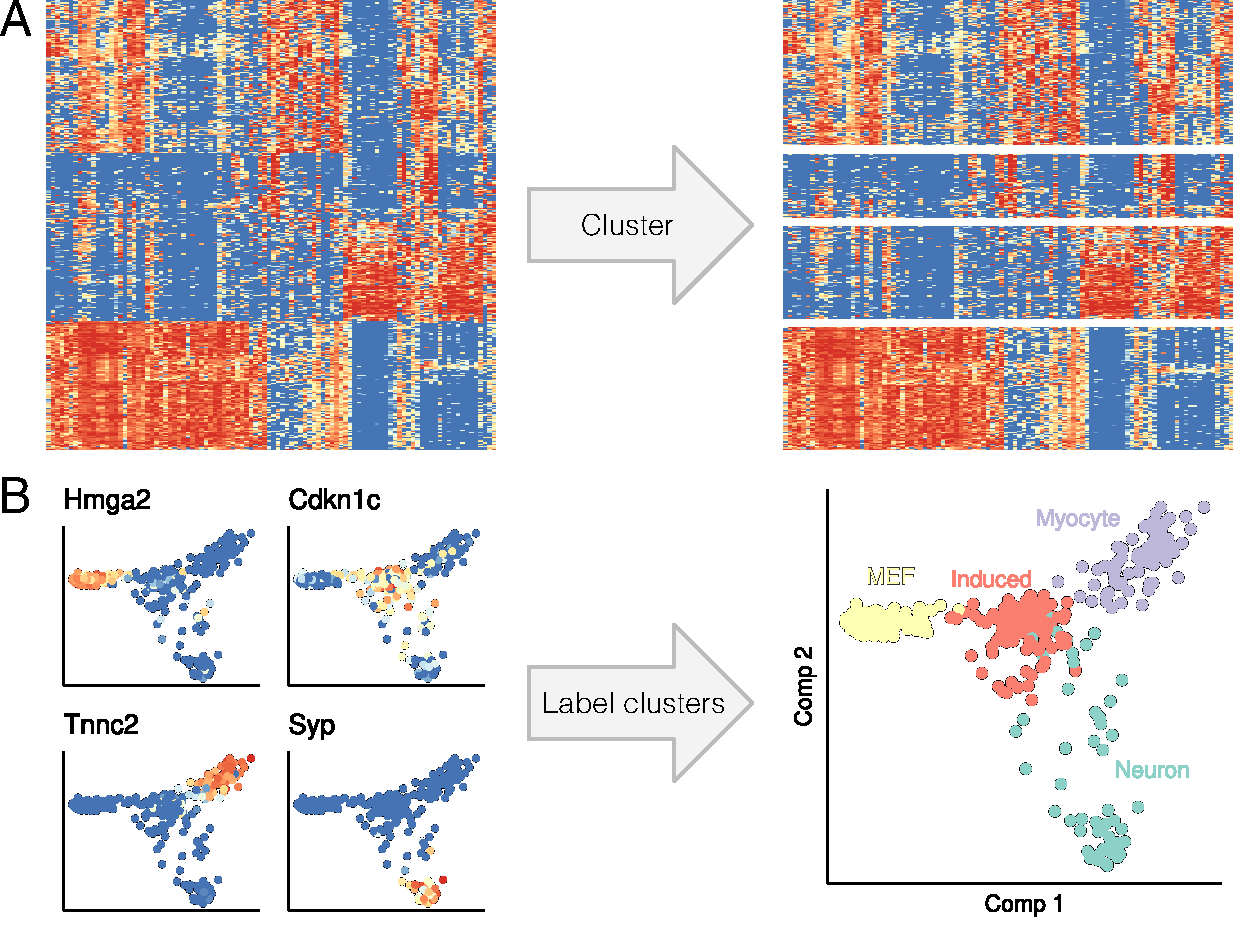
\includegraphics[width=.6\linewidth]{fig/comptools2/comptool_2_clustering.pdf} 
	\caption{
		\textbf{Clustering for single-cell omics data.}
		\textbf{A:} Clustering methods group cells with similar omics profiles together. 
		\textbf{B:} By overlaying gene expression levels on a dimensionality reduction, the clusters can be annotated to allow better interpretation of the cellular heterogeneity.
	}
	\label{fig:comp_tools_cluster}
\end{figure}


Usually, the number of clusters is determined by the user, either as a direct parameter (e.g. $k$-means\cite{lloyd_leastsquaresquantization_1982}) or an indirect parameter (e.g. a height cutoff in hierarchical clustering). In some exceptional cases, the number of clusters is strictly determined by the data itself and cannot be altered with a parameter (e.g. Louvain clustering\cite{blondel_fastunfoldingcommunities_2008}).

Clustering methods used in this work are mostly restricted to $k$-Means for clustering low-dimensional spaces and Louvain for clustering networks, since both are highly scalable with respect to the number of cells.

\subsection{Trajectory inference}
While clustering methods divide cells into distinct groups, trajectory inference (TI) methods acknowledge that cells are dynamic entities which transition from once cellular state to another via various dynamic processes. Rather than making distinct groups, TI methods allow studying dynamic processes by reconstructing the topology of a dynamic process as a trajectory, and map the cells onto that trajectory (Figure~\ref{fig:comp_tools_ti}A). Similar to clustering, by colouring the cells according to the expression of genes known to be involved in the dynamic process of interest, the milestones in the trajectory can be annotated (Figure~\ref{fig:comp_tools_cluster}B). 


\begin{figure}[htb!]
	\centering
	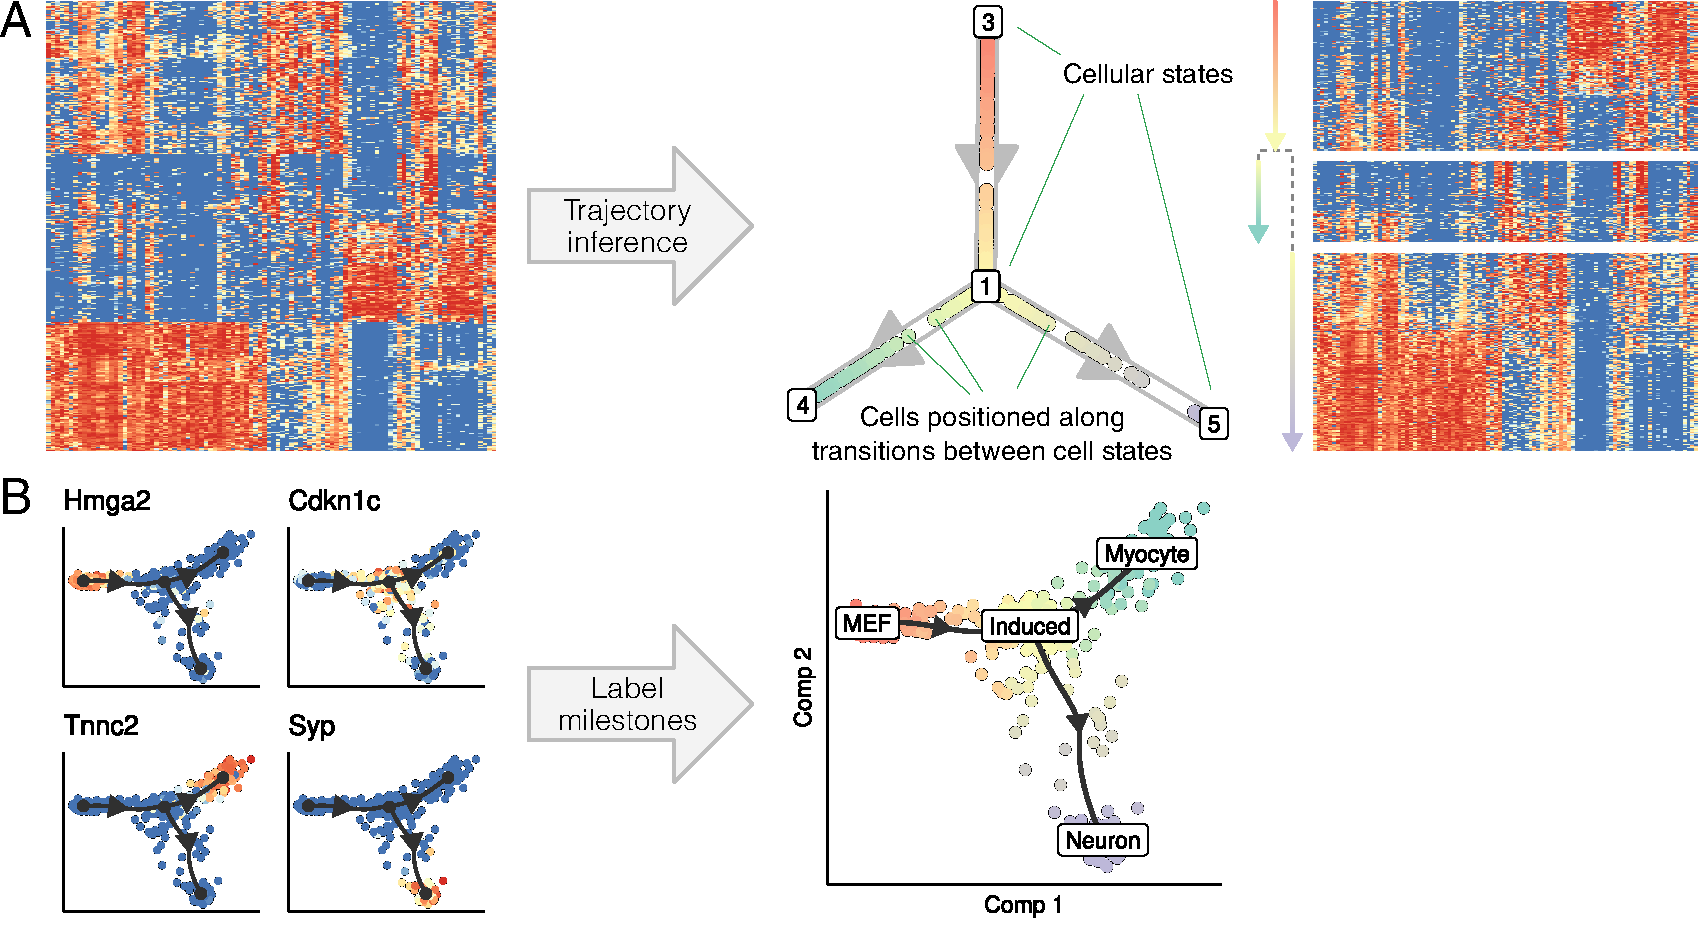
\includegraphics[width=.6\linewidth]{fig/comptools2/comptool_3_trajectoryinference.pdf} 
	\caption{
		\textbf{Trajectory inference for single-cell omics data.}
		\textbf{A:} During a dynamic process cells pass through several transitional states, characterized by different waves of transcriptional, morphological, epigenomic and/or surface marker changes\cite{enver_stemcellstates_2009}. TI methods provide a straightforward and unbiased approach to identifying and correctly ordering different transitional stages. 
		\textbf{B:} By overlaying gene expression levels on a dimensionality reduction, the milestones can be annotated to allow better interpretation of the cellular heterogeneity.
	}
	\label{fig:comp_tools_ti}
\end{figure}

TI methods typically first require some form of dimensionality reduction prior to inferring a trajectory from the dataset (Figure~\ref{fig:ti_metro}). Subsequently, a trajectory modelling step then operates in this reduced space, aiming to identify cell states, constructing a trajectory through the different states, and projecting the cells back on to the trajectory. 

A common way to classify TI methods is by the types of trajectories they can infer\cite{saelens_comparisonsinglecelltrajectory_2019}. About half of TI methods specialise in inferring linear or cyclic trajectories (i.e. they order the cells). Others model the trajectory as a rooted tree, allowing for one or more bifurcations to occur. Only a few methods are able to infer more generalised trajectories containing disconnected subgraphs or cycles.

\begin{figure}[htb!]
	\centering
	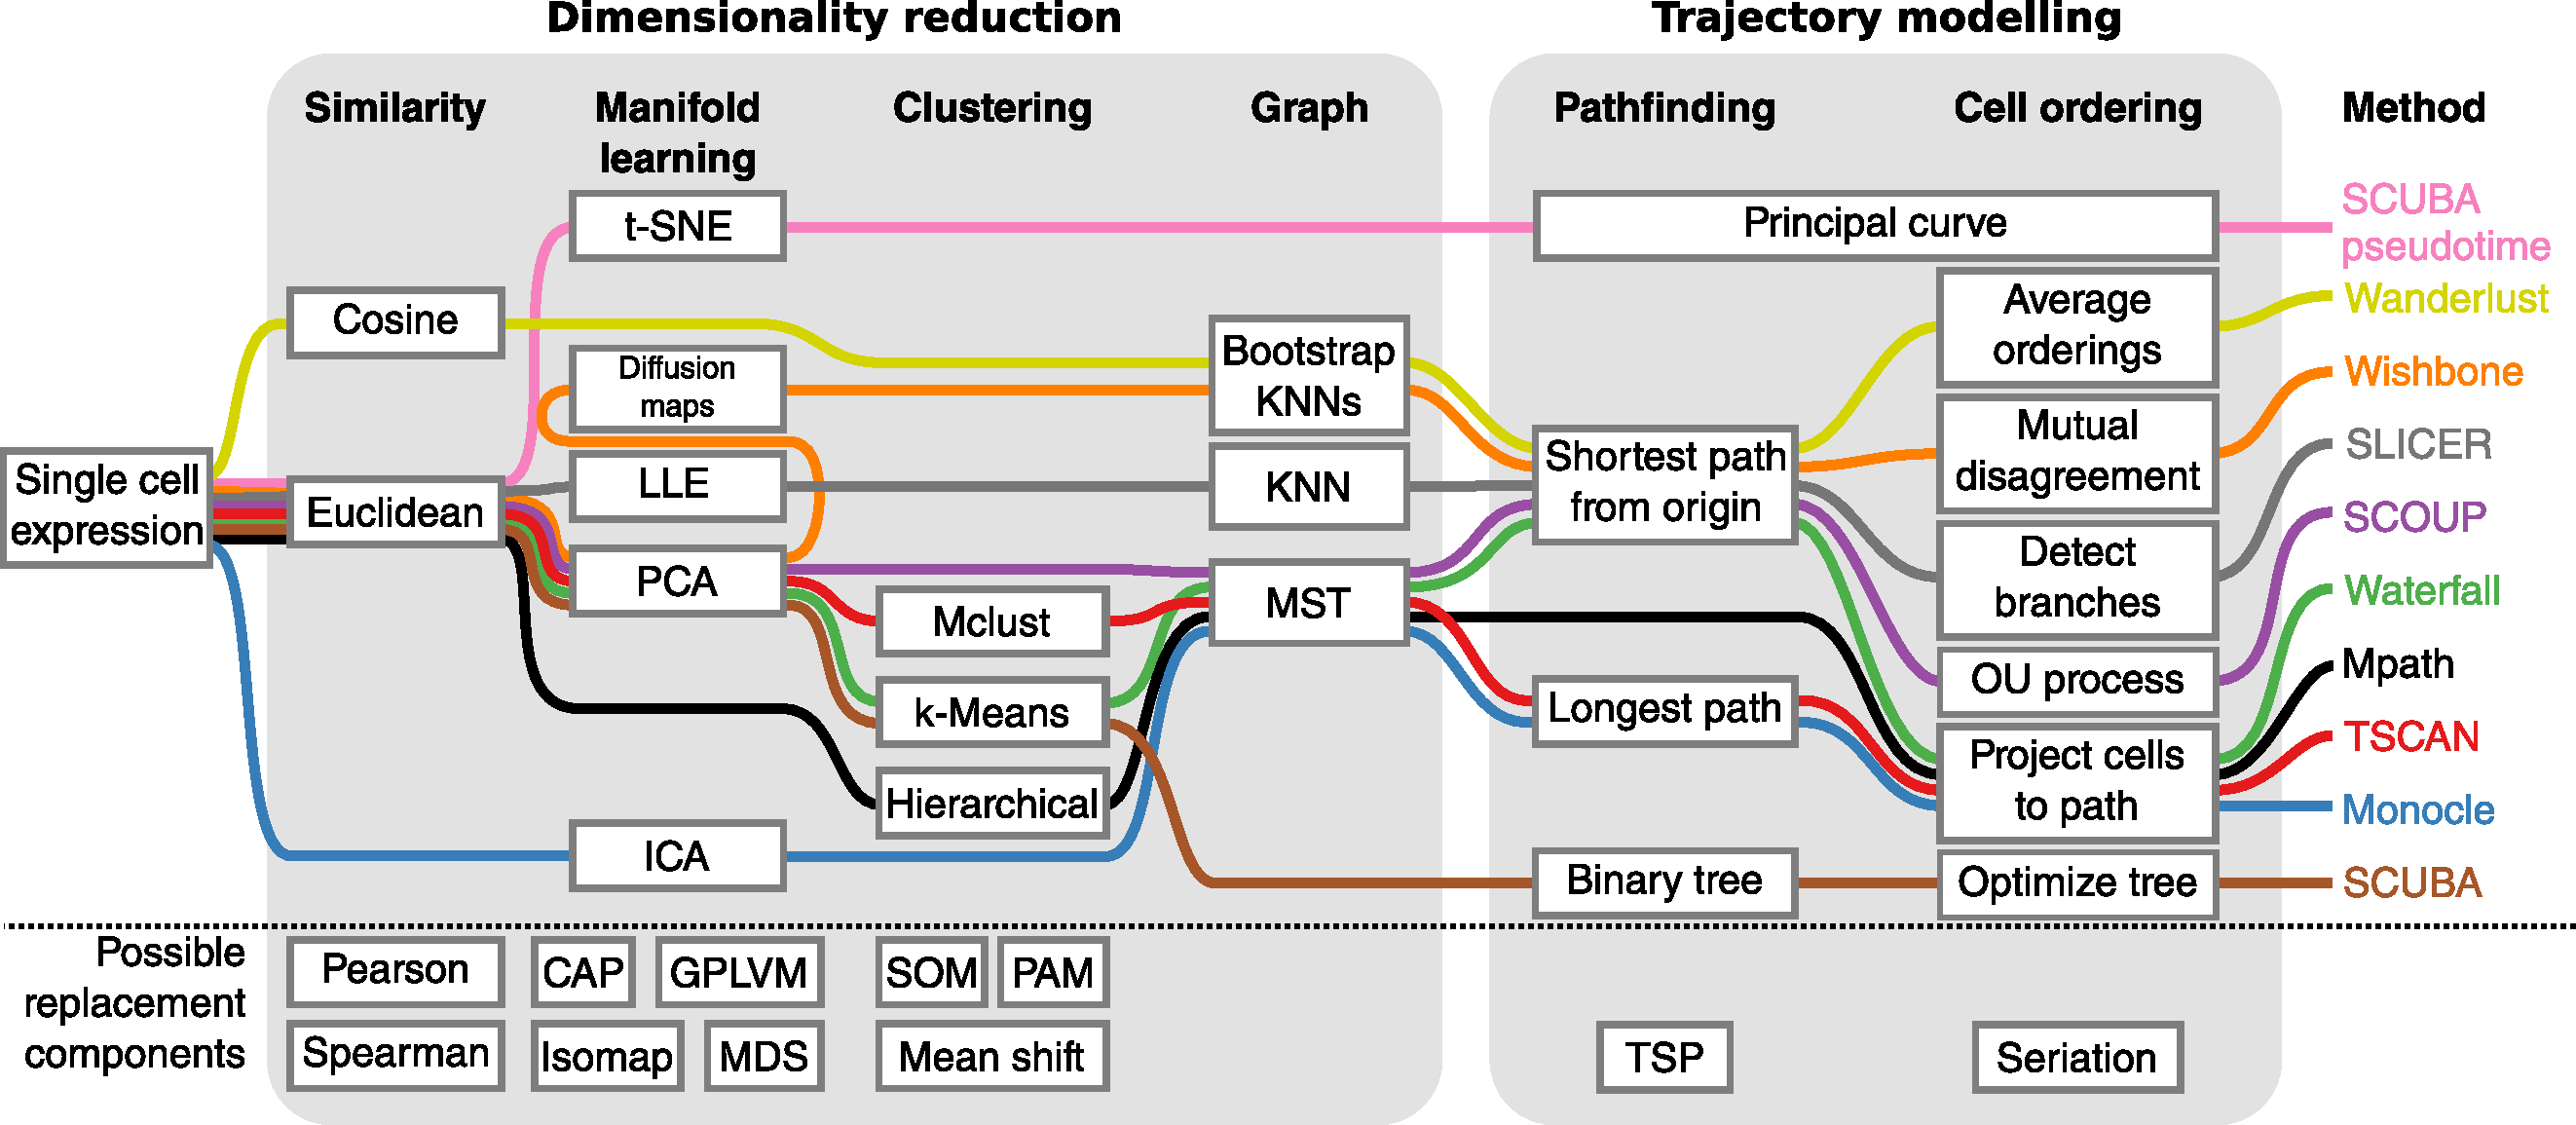
\includegraphics[width=.9\linewidth]{fig/ti_metro} 
	\caption{
		\textbf{TI methods use several common building blocks and can be organized in a unifying modular framework.} Overall, TI consists of two steps. In the first step dimensionality reduction techniques such as manifold learning, clustering, or graph-based methods are used to convert the dataset to a more simplified representation. This representation of the data then allows the trajectory itself to be more easily modelled in a second step. In this step, the trajectory itself is found within the data using both graph-based and curve-based approaches, after which the cells themselves can be ordered using a variety of methods.
	}
	\label{fig:ti_metro}
\end{figure}


\subsection{Differential expression}
Given that cells are split up into groups differential expression (DE) methods ranks genes based on whether their expression is significantly higher or lower in one group in comparison to the others. This grouping can be based on prior information or an upstream clustering method. DE methods are useful for summarising the main differences between different groups of cells more compactly (Figure~\ref{fig:comp_tools_de}A) in comparison to when groups are compared without gene prioritisation (Figure~\ref{fig:comp_tools_cluster}A). 

Trajectory differential expression (TDE) is an extension of DE where instead genes are prioritised according to whether their gene expression changes smoothly but significantly along a parts of a trajectory (Figure~\ref{fig:comp_tools_de}). 

\begin{figure}[htb!]
	\centering
	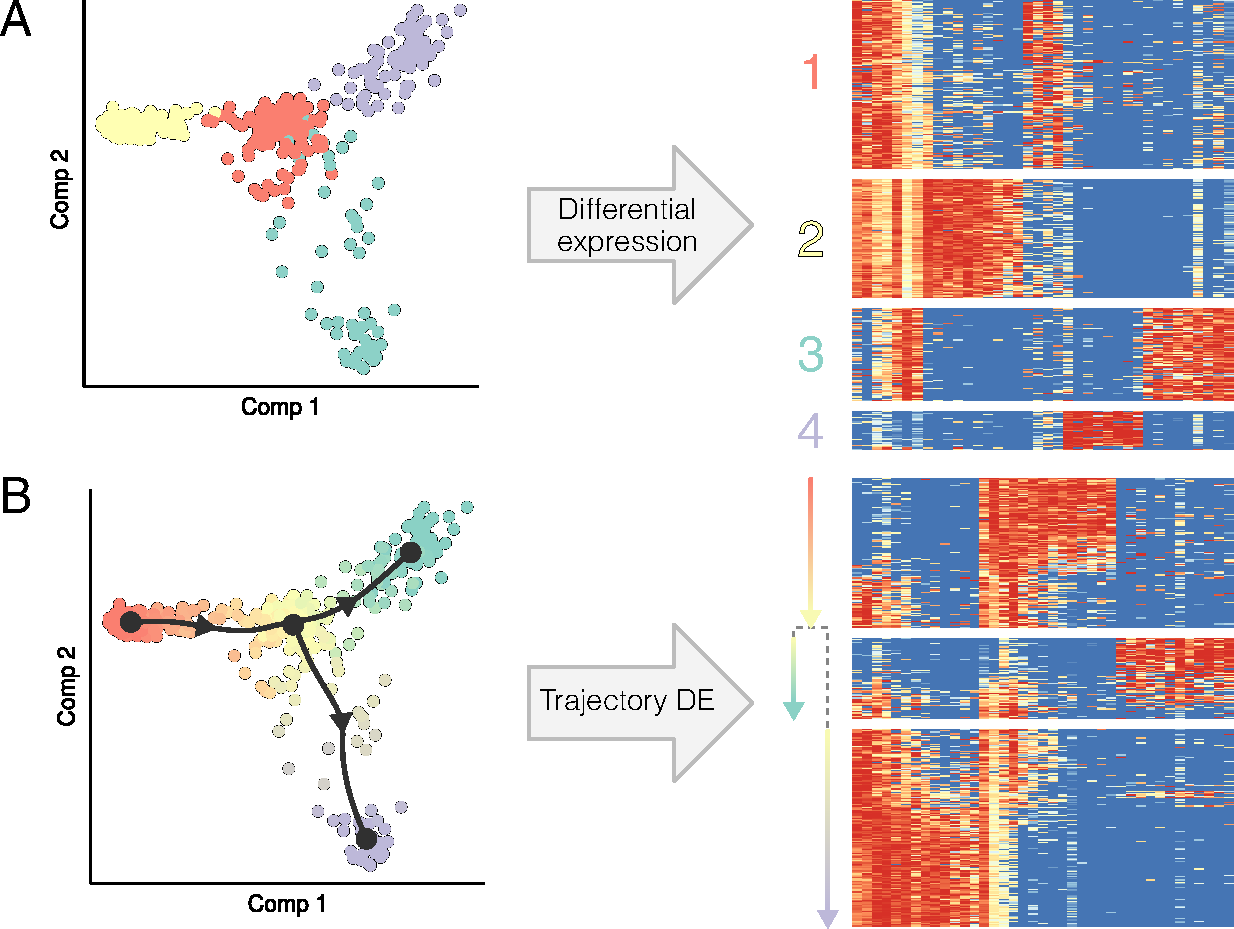
\includegraphics[width=.6\linewidth]{fig/comptools2/comptool_4_differentialexpression.pdf} 
	\caption{
		\textbf{Differential expression for single-cell omics data.}
		\textbf{A:} Differential expression methods prioritises genes that are expressed significantly higher or lower in particular given groups.
		\textbf{B:} Trajectory differential expression prioritises genes that change smoothly but significantly along particular transitions in a trajectory.
	}
	\label{fig:comp_tools_de}
\end{figure}

\subsection{Network inference}
One of the central cellular processes underlying development is transcriptional regulation. 	
Modeling the dynamics of gene regulation is therefore essential to better understand why a cellular dynamic processes progresses through several steps, and what goes wrong in the case of disease.

Network inference (NI) methods predict which genes are regulated by which transcription factors (Figure~\ref{fig:comp_tools_ni}). Before single-cell omics, these methods rely on multiple experiments, amongst which perturbation and time-series experiments, to predict the effect each transcription factor has on the up- or downregulation of a gene. 

One of the main advantages of single-cell omics is the heterogeneity between cells caused by naturally occurring biological randomness\cite{padovan-merhar_usingvariabilitygene_2013} can be exploited to infer regulatory interactions between TFs and their target genes at much lower costs. 

\begin{figure}[htb!]
	\centering
	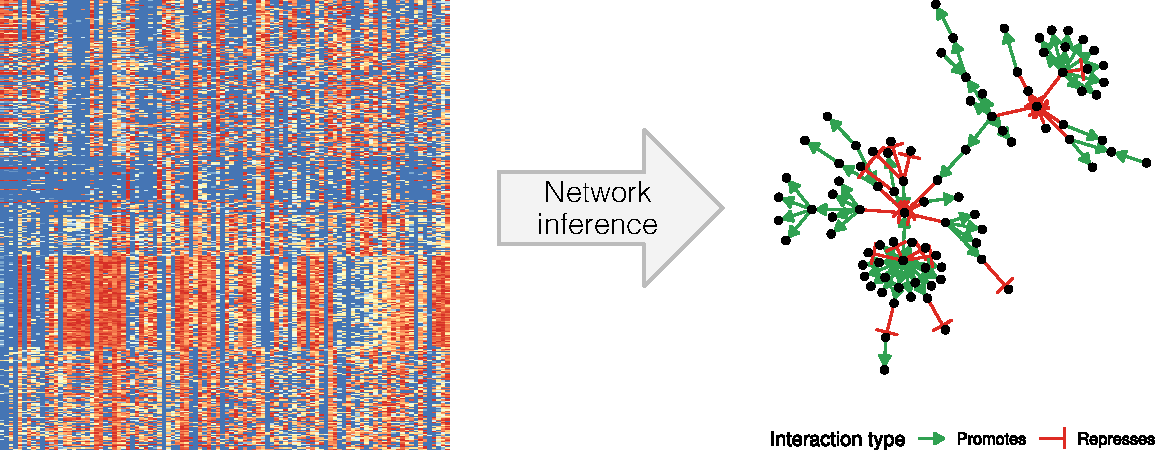
\includegraphics[width=.6\linewidth]{fig/comptools2/comptool_5_networkinference.pdf}
	\caption{
		\textbf{Network inference for single-cell omics data.}
	}
	\label{fig:comp_tools_ni}
\end{figure}



\section{Research context and objectives}
Recent technological advancements in profiling single cells are having significant repercussions in many fields of biology. Profiling thousands of individual cells in a genome-wide manner provides opportunities to study cell heterogeneity and dynamics, for example inferring mechanisms for cellular development or intercellular communication. 
Hundreds of new software tools were developed\cite{zappia_exploringsinglecellrnaseq_2018} to perform these new types of analyses, or to fit existing analytical tools to deal with new data characteristics (e.g. differential expression, dimensionality reduction, normalisation). 

One major shortcoming during the advent of single-cell omics was that majority of the newly developed computational tools were not quantitatively and comparatively evaluated. Rather, they relied on anecdotal evidence to demonstrate its usefulness. This issue is not the result of the tool developer's malevolence, but instead of the lack of data required to perform such comprehensive benchmarks.
%TODO: also mention guidelines for users.

Uncontrolled development of software tools without comprehensive benchmarking poses serious problems. 
For one, it slows down scientific progress. Every end-user needs to make a large commitment researching the domain in order to make an informed decision of which tool to use, or risk a higher incidence of false positive discoveries (either way, valuable resources are being wasted). In addition, it also negatively impacts the credibility of the field, thus discouraging potential users or researchers from entering.

In this work, we aim to speed up scientific progress in single-cell omics by providing tools both for end-users and developers alike. For developers of computational approaches, we provide tools and guidelines for benchmarking their method on real and synthetic data. For end-users we develop new tools and guidelines for analysing dynamic processes by inferring trajectories and gene regulatory networks. These contributions are discussed in the following chapters:

\begin{itemize}
	\item We develop benchmarking strategies for assessing the performance of computational tools constrained by low availability of novel types of real single-cell data (Chapter~\ref{chap:dyngen}). \textit{In silico} simulations of individual cells are used to help kick-start emerging domains much more safely and allow anticipation of future technological developments by already developing computational tools.
	\item We apply this strategy to perform a comparison of TI methods (Chapter~\ref{chap:dynbenchmark}). Trajectory inference is one of the largest categories of all the novel single-cell omics tools, yet a comprehensive and quantitative study of the advantages and disadvantages of the numerous tools was hitherto lacking. We provide a set of guidelines for end-users wishing to infer trajectories. We also make our pipeline, datasets, metrics, and containerised wrappers of TI methods publicly available for developers to use.
	\item We developed dyno, a toolkit to easily infer, visualise and interpret single-cell trajectories using more than 50 different TI methods (Chapter~\ref{chap:dyno}). dyno provides downstream analysis such as: visualising a trajectory in a low-dimensional space or a heatmap, detecting genes differentially expressed at different stages of the tragectory, comparing multiple trajectories in a common dimensionality reduction, and manipulating the trajectory (e.g. adding directionality or adding annotation).
	\item We introduce a novel TI method specialised in inferring linear trajectories (Chapter~\ref{chap:scorpius}). Despite linear TI being the most simple but commonly used form of trajectory inference, the benchmark demonstrated that most TI methods are not capable of producing accurate models of linear datasets.
	\item We invent a new type of NI method capable of inferring the GRN of individual cells (Chapter~\ref{chap:bred}). We demonstrate this <yadeyade .. fill in when the chapter is actually written.>
	% TODO: fill this part in!!!
	\item Every NI method has certain topological biases. We provide a tool for analysing the topological properties of large, evolving networks and use this to iteratively optimise GRN predictions (Chapter~\ref{chap:incgraph}).
	\item We discuss reproducibility problems of TI methods due to low rates of quantitative self-assessment (Chapter~\ref{chap:selfassessment}). We provide solutions for different causal reasons for this phenomenon in order to spur developers to perform more self-assessments.
	\item Finally, we summarise our experience in benchmarking computational methods in a list of essential guidelines (Chapter~\ref{chap:guidelines}).
\end{itemize}


\section{List of contributions}

\subsection{First-author publications}

\begin{itemize}
	\item \textbf{Cannoodt R} *, Saelens W *, Saeys Y. Computational methods for trajectory inference from single-cell transcriptomics. European journal of immunology. 2016 Nov;46(11):2496-506.
	\item \textbf{Cannoodt R}, Ruyssinck J, Ramon J, De Preter K, Saeys Y. IncGraph: Incremental graphlet counting for topology optimisation. PloS one. 2018 Apr 26;13(4):e0195997.
	\item Saelens W *, \textbf{Cannoodt R} *, Todorov H, Saeys Y. A comparison of single-cell trajectory inference methods. Nature biotechnology. 2019 May;37(5):547.
	\item \textbf{Cannoodt R}, Saelens W, Sichien D, Tavernier S, Janssens S, Guilliams M, Lambrecht B, De Preter K, Saeys Y. SCORPIUS: Fast, accurate, and robust single-cell pseudotime. In preparation.
	\item \textbf{Cannoodt R} *, Saelens W *, Saeys Y. dyngen: Simulating developing single cells. In preparation.
	\item \textbf{Cannoodt R} *, Saelens W *, Saeys Y. dyno: A toolkit for inferring, visualising, and interpreting trajectories. In preparation.
	\item \textbf{Cannoodt R}, Saelens W, Saeys Y, De Preter K. bred: Inferring single cell regulatory networks. In preparation. \fbox{\color{red}order authors?}
	\item \textbf{Cannoodt R}, Saelens W, Saeys Y. Self-assessment in trajectory inference. In preparation.
\end{itemize}

*: Equal contribution.

\subsection{Co-author publications}
\begin{itemize}
	\item Decock A, Ongenaert M, \textbf{Cannoodt R}, Verniers K, De Wilde B, Laureys G, Van Roy N, Berbegall AP, Bienertova-Vasku J, Bown N, Clément N. Methyl-CpG-binding domain sequencing reveals a prognostic methylation signature in neuroblastoma. Oncotarget. 2016 Jan 12;7(2):1960.
	\item Van Cauwenbergh C, Van Schil K, \textbf{Cannoodt R}, Bauwens M, Van Laethem T, De Jaegere S, Steyaert W, Sante T, Menten B, Leroy BP, Coppieters F. arrEYE: a customized platform for high-resolution copy number analysis of coding and noncoding regions of known and candidate retinal dystrophy genes and retinal noncoding RNAs. Genetics in Medicine. 2017 Apr;19(4):457.
	\item Claeys S, Denecker G, \textbf{Cannoodt R}, Kumps C, Durinck K, Speleman F, De Preter K. Early and late effects of pharmacological ALK inhibition on the neuroblastoma transcriptome. Oncotarget. 2017 Dec 5;8(63):106820.
	\item Depuydt P, Boeva V, Hocking TD, \textbf{Cannoodt R}, Ambros IM, Ambros PF, Asgharzadeh S, Attiyeh EF, Combaret V, Defferrari R, Fischer M. Genomic amplifications and distal 6q loss: novel markers for poor survival in high-risk neuroblastoma patients. JNCI: Journal of the National Cancer Institute. 2018 Mar 5;110(10):1084-93.
	\item Scott CL, T'Jonck W, \ldots, \textbf{Cannoodt R}, Saelens W \ldots, Guilliams M. The transcription factor ZEB2 is required to maintain the tissue-specific identities of macrophages. Immunity. 2018 Aug 21;49(2):312-25.
	\item Saelens W, \textbf{Cannoodt R}, Saeys Y. A comprehensive evaluation of module detection methods for gene expression data. Nature communications. 2018 Mar 15;9(1):1090.
	\item Todorov H, \textbf{Cannoodt R}, Saelens W, Saeys Y. Network Inference from Single-Cell Transcriptomic Data. In Gene Regulatory Networks 2019 (pp. 235-249). Humana Press, New York, NY..
	\item Van den Berge K, De Bezieux HR, Street K, Saelens W, \textbf{Cannoodt R}, Saeys Y, Dudoit S, Clement L. Trajectory-based differential expression analysis for single-cell sequencing data. BioRxiv. 2019 Jan 1:623397.
	\item Weber LM, Saelens W, \textbf{Cannoodt R}, Soneson C, Hapfelmeier A, Gardner PP, Boulesteix AL, Saeys Y, Robinson MD. Essential guidelines for computational method benchmarking. Genome biology. 2019 Dec;20(1):125.
	\item Lorenzi L, \ldots, \textbf{Cannoodt R}, \ldots, Mestdagh P. The RNA-Atlas, a single nucleotide resolution map of the human transcriptome. In preparation.
	\item Van den Berge K, Roux de Bézieux H, Street K, Saelens W, \textbf{Cannoodt R}, Saeys Y, Dudoit S. Trajectory-based differential expression analysis. Submitted to Nature Communications.
	\item Van de Sande Bram, \ldots, \textbf{Cannoodt R}, \ldots, Saeys Y, Aerts S. A scalable SCENIC workflow for single-cell gene regulatory network analysis. Submitted to Nature Protocols.
\end{itemize}

\subsection{Open-source software}
As part of this work, many open-source software packages were created and many others were contributed to (Table \ref{tab:packages}). 

Packages that were created as part of this work are hosted on Github under the username rcannood\footnote{\url{https://github.com/rcannood?tab=repositories}} or the dynverse organisation\footnote{\url{https://github.com/dynverse?tab=repositories}}. As part of our standard development practices, we automate execution of unit tests and writing extensive documentation to ensure the code complies with CRAN policy before submission. We aim to submit all other packages to CRAN as well.

We also helped maintain or extend other packages on Github, CRAN or Bioconductor on which our software depends. This includes speeding up parts of the dependency (slingshot), adding new functionality (devtools, ParamHelpers), fixing bugs (proxyC, rlang, monocle, splatter, slingshot), becoming a maintainer of orphaned packages (diffusionMap, princurve, GillespieSSA), and extending the documentation (devtools, mlr, remotes). Several of these package receive millions of downloads per year (devtools, remotes, rlang).

\newcommand{\cranpkg}[1]{\href{https://cran.r-project.org/package=#1}{#1}}
\newcommand{\biocpkg}[1]{\href{https://bioconductor.org/packages/#1}{#1}}
\newcommand{\biocpkgl}[2]{\href{https://bioconductor.org/packages/#1}{#2}}
\newcommand{\githubpkg}[2]{\href{https://github.com/#1/#2}{#2}}
\newcommand{\notavailable}{}

\begin{table}[ht!]
	\caption{\textbf{Contibutions to open-source software.} Following abbreviations denote the relation with respect to the package: \textit{aut} Author, \textit{ctb} Contributor. Yearly download statistics are based on the number of downloads between 2019-08-01 and 2019-09-10. CRAN download statistics are retrieved from the Rstudio CRAN mirror only; other CRAN mirrors do not track download statistics. In addition, many of the dynverse packages have only recently been published on CRAN. For Github repositories, no download statistics could be retrieved. } \label{tab:packages}
	
	\centering\fontsize{9}{11}\selectfont
	\begin{tabularx}{\linewidth}{|p{2cm}llp{1.5cm}X|}
		\hline
		Name & Role & Host & Downloads per year & Description \\ \hline\hline
		\cranpkg{babelwhale} & aut & CRAN & 5810 & Interacting with Docker and Singularity containers \\
		\cranpkg{diffusionMap} & aut & CRAN & 30'450 & Implements diffusion map method of data parameterization, including creation and visualization of diffusion map \\
		\githubpkg{dynverse}{dynbenchmark} & aut & Github & \notavailable & Pipeline for benchmarking trajectory inference methods \\
		\cranpkg{dyndimred} & aut & CRAN & 5535 & Applying dimensionality reduction methods \\
		\githubpkg{dynverse}{dyneval} & aut & Github & \notavailable & Evaluating trajectory inference methods \\
		\githubpkg{dynverse}{dynfeature} & aut & Github & \notavailable & Calculating feature importance scores from trajectories \\
		\githubpkg{dynverse}{dyngen} & aut & Github & \notavailable & Simulating single-cell data using gene regulatory networks \\
		\githubpkg{dynverse}{dynguidelines} & aut & Github & \notavailable & User guidelines for trajectory inference \\
		\githubpkg{dynverse}{dynmethods} & aut & Github & \notavailable & A collection of wrappers for trajectory inference methods \\
		\githubpkg{dynverse}{dyno} & aut & Github & \notavailable & A pipeline for inferring, visualising and interpreting trajectories \\
		\cranpkg{dynparam} & aut & CRAN & 3265 & Creating meta-information for parameters \\
		\githubpkg{dynverse}{dynplot} & aut & Github & \notavailable & A simple visualisation library for trajectories \\
		\githubpkg{dynverse}{dynplot2} & aut & Github & \notavailable & A fully customisable visualisation library for trajectories \\
		\githubpkg{dynverse}{dyntoy} & aut & Github & \notavailable & Generating simple toy data of cellular differentiation \\
		\cranpkg{dynutils} & aut & CRAN & 13'13' & Common functionality for the dynverse packages \\
		\cranpkg{dynwrap} & aut & CRAN & 990 & A common format for trajectories \\
		\cranpkg{GillespieSSA} & aut & CRAN & 7880 & Gillespie's Stochastic Simulation Algorithm (SSA) \\
		\cranpkg{GillespieSSA2} & aut & CRAN & 4950 & Gillespie's Stochastic Simulation Algorithm for Impatient People \\
		\githubpkg{dynverse}{gng} & aut & Github & \notavailable & An Rcpp implementation of the Growing Neural Gas algorithm \\
		\cranpkg{incgraph} & aut & CRAN & 3565 & Incremental graphlet counting for network optimisation \\
		\cranpkg{lmds} & aut & CRAN & 815 & Landmark Multi-Dimensional Scaling \\
		\cranpkg{princurve} & aut & CRAN & 29'100 & Fits a principal curve in arbitrary dimension \\
		\cranpkg{proxyC} & aut & CRAN & 117'480 & Computes proximity in large sparse matrices \\
		\cranpkg{qsub} & aut & CRAN & 3585 & Running commands remotely on gridengine clusters \\
		\cranpkg{SCORPIUS} & aut & CRAN & 4520 & Inferring developmental chronologies from single-cell RNA sequencing data \\ \hline\hline
		
		\cranpkg{badger} & ctb & CRAN & 6240 & Query information and generate badge for using in README and GitHub Pages \\
		\biocpkgl{ClusterSignificance}{Clus\-ter\-Sig\-nif\-i\-cance} &  & Bioc & 935 & Assess if class clusters in dimensionality reduced data representations have a separation different from permuted data \\
		\cranpkg{devtools} & ctb & CRAN & 5'918'700 & Tools to make developing R packages easier \\
		\githubpkg{soedinglab}{merlot} & ctb & Github & \notavailable & A method for reconstructing lineage-tree topologies from scRNA-seq data \\
		\cranpkg{mlr} & ctb & CRAN & 176'330 & Machine Learning in R \\
		\biocpkg{monocle} & ctb & Bioc & 34'360 & Clustering, differential expression, and trajectory analysis for single-cell RNA-Seq \\
		\cranpkg{ParamHelpers} & ctb & CRAN & 150'775 & Helpers for Parameters in Black-Box Optimization, Tuning and Machine Learning \\
		\githubpkg{kieranrcampbell}{pseudogp} & ctb & Github & \notavailable & Probabilistic pseudotime for single-cell RNA-seq \\
		\cranpkg{Rdimtools} & ctb & CRAN & 7367 & Dimension Reduction and Estimation Methods \\
		\cranpkg{remotes} & ctb & CRAN & 3'944'090 & R package installation from remote repositories, including GitHub \\
		\cranpkg{rlang} & ctb & CRAN & 13'269'115 & Functions for base types and core R and tidyverse features \\
		\githubpkg{aertslab}{SCope} & ctb & Github & \notavailable & Visualization of large-scale and high dimensional single cell data \\
		\biocpkg{slingshot} & ctb & Bioc & 12'085 & Tools for ordering single-cell sequencing \\
		\biocpkg{splatter} & ctb & Bioc & 5015 & Simple simulation of single-cell RNA sequencing data \\
		\githubpkg{farrelja}{URD} & ctb & Github & \notavailable & URD reconstructs transcriptional trajectories underlying specification or differentiation processes in the form of a branching tree from single-cell RNAseq data \\
		\githubpkg{ManuSetty}{wishbone} & ctb & Github & \notavailable & Identify bifurcating developmental trajectories from single-cell data \\\hline
	\end{tabularx}
\end{table}
